\chapter{Ergebnisse und Diskussion}

\section{Leistungsmessung}

\subsection{Gesamtprogramm}

Messungen des Gesamtprogramms (Datentransfers, alle Stufen)

\subsection{Teilstufen}

grobe Messungen der Teilstufen (Wichtung, Filterung, Rückprojektion)

Ergebnis: Rückprojektion braucht am längsten

\subsection{Eigenschaften des Rückprojektionskernels}

In Abschnitt~\ref{ssec:opti_ueber} wurde als Implementierungsziel unter anderem eine möglichst hohe \gls{gpu}-Auslastung
gefordert. Um diese Auslastung zu erreichen, ist ein möglichst geringer Verbrauch der zwischen den Threads geteilten
Ressourcen erforderlich. Da der \textit{Shared Memory} in der Implementierung nicht verwendet wurde, zielte die
Umsetzung dieser Forderung auf einen möglichst geringen Registerverbrauch ab.

Wie in Abbildung~\ref{fig:kernel_props} zu sehen ist, benötigt der Rückprojektions-\gls{kernel} 19 Register
(grün markiert). Auf der hier verwendeten GeForce GTX 1080 ist somit eine theoretische Auslastung der gesamten \gls{gpu}
möglich, praktisch wird die \gls{gpu} durch die Rückprojektion zu 88,5\% ausgelastet (rot markiert).

Ein weiteres der drei Optimierungsziele, die in Abschnitt~\ref{ssec:opti_ueber} genannt wurden, ist die Verkürzung der
Wartezeit zwischen dem Ende einer Rückprojektion und dem Beginn der nachfolgenden Rückprojektion. Zu diesem Zweck wird
die Rückprojektion in einem eigenen Thread und \gls{cuda}-Stream ausgeführt, sodass die vorherigen Operationen (Laden,
Wichten, Filtern) parallel zur Rückprojektion ausgeführt werden können. Der Rückprojektionsthread entnimmt die nächste
Projektion vom Stapel der noch ausstehenden Projektionen, wandelt diese in eine \gls{cuda}-Textur um und startet dann
den Rückprojektions-\gls{kernel}. Wie Abbildung~\ref{fig:kernel_wait} zeigt, ist es gelungen, die Zeit zwischen zwei
Rückprojektionen, die durch die langen, grün-blauen Balken dargestellt werden, auf 2 Millisekunden zu beschränken. Bei
einem üblichen Datensatz von 1440 Projektionen ergibt sich also eine Gesamtwartezeit von 2,88 Sekunden.

Abbildung~\ref{fig:kernel_wait} zeigt allerdings auch, dass diese Wartezeit noch nicht ideal ist. Das Ziel, die Wichtung
und die Filterung, die durch die kleineren, bunten Balken repräsentiert werden, parallel zur Rückprojektion
durchzuführen, konnte nicht erreicht werden. Der Grund dafür ist vermutlich die Anzahl der Threads, die vom
Rückprojektions-\gls{kernel} gestartet werden. Bei einem Volumen mit 1070 x 1070 x 1033 \gls{voxel}n, denen jeweils ein
Thread zugeordnet wird, werden 1.182.681.700 Threads benötigt. Die GTX 1080 verfügt über 20 \gls{sm}s, von denen jeder
bis zu 2.048 Threads gleichzeitig ausführen kann und kann somit bis zu 40.960 Threads gleichzeitig verwalten. Die
\gls{gpu} ist daher gezwungen, der Rückprojektion alle verfügbaren Threads zuzuweisen, was zur Folge hat, dass keine
weiteren \gls{kernel} ausgeführt werden können. Wenn auch die parallele Ausführung der Rückprojektion und der vorherigen
Schritte nicht gelungen ist, ist auf der Abbildung jedoch zu sehen, dass die Ausführung der \gls{kernel} mit geringerem
Ressourcenbedarf sich stellenweise überlappt.

Die Wartezeit zwischen zwei Rückprojektionen, die über die gesamte Laufzeit akkumuliert ca. 3 Sekunden einnimmt, hat
also einen akzeptablen Wert erreicht, der dem alltäglichen Gebrauch nicht im Wege steht. Auch wenn an dieser Stelle noch
Optimierungspotential vorhanden ist, wäre selbst eine vollständige Eliminierung der Wartezeit vernachlässigbar.

\begin{figure}
    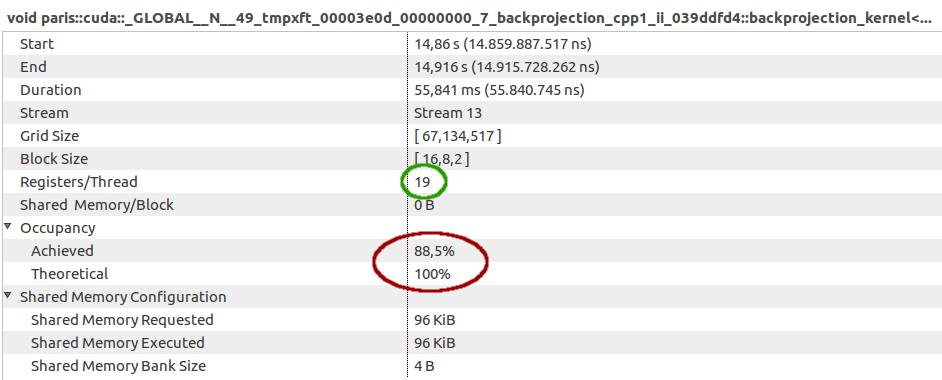
\includegraphics[width=\linewidth]{img/kernel_properties}
    \caption{Eigenschaften des Rückprojektionskernels}
    \label{fig:kernel_props}
\end{figure}

\begin{figure}
    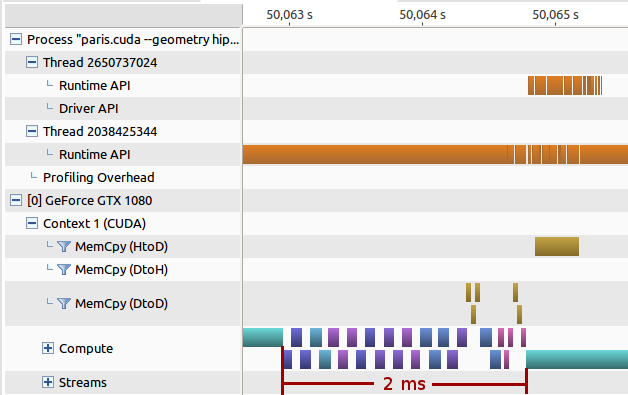
\includegraphics[width=\linewidth]{img/timeline_compute3}
    \caption{Zeit zwischen zwei Rückprojektionen}
    \label{fig:kernel_wait}
\end{figure}

\subsection{Laufzeitverhalten}

Die parallele Berechnung verschiedener Teile des Volumens durch den Einsatz mehrerer \gls{gpu}s war ebenfalls ein
Implementierungsziel. Die besondere Herausforderung bestand darin, sowohl mehrere \gls{gpu}s des gleichen Typs als auch
unterschiedliche \gls{gpu}s zu unterstützen.

Wie Abbildung~\ref{fig:kernel_multi_compute} zeigt, ist es gelungen, die Ausführung parallel auf mehreren \gls{gpu}s
durchzuführen. Der gewählte Ansatz zur Lastverteilung (siehe Abschnitt~\ref{}) führt jedoch bei unterschiedlich
leistungsstarken \gls{gpu}s dazu, dass die stärkere \gls{gpu} vor der schwächeren fertig ist und dann auf diese warten
muss, wie in Abbildung~\ref{fig:kernel_multi_bad} zu sehen ist.

In Abbildung~\ref{fig:laufzeit_gpus} ist das Laufzeitverhalten unterschiedlicher \gls{gpu}s dargestellt. Es ist klar
zu sehen, dass der gemeinsame Einsatz der Tesla K20c und der GTX 1080 in diesem Fall sogar zu einer längeren Laufzeit
führt, als der alleinige Einsatz der GTX 1080. Die statische Lastverteilung, wie sie in dieser Arbeit beschrieben ist,
sollte daher zukünftig auf heterogenen \gls{gpu}-Systemen durch andere Methoden abgelöst werden. Denkbar ist
beispielsweise der Einsatz von \textit{Machine-Learning}-Techniken, durch die die optimale Lastverteilung iterativ
ermittelt wird.

\begin{figure}
    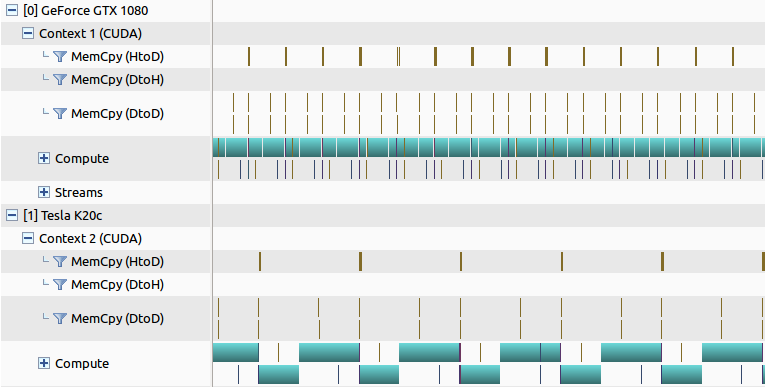
\includegraphics[width=\linewidth]{img/timeline_multi_compute}
    \caption{Parallele Ausführung auf zwei \gls{gpu}s}
    \label{fig:kernel_multi_compute}
\end{figure}

\begin{figure}
    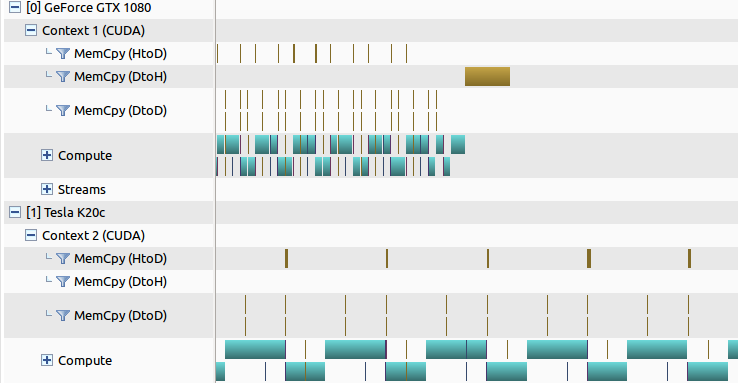
\includegraphics[width=\linewidth]{img/timeline_multi_bad}
    \caption{Der gewählte, statische Lastverteilungsansatz führt zu Wartezeiten}
    \label{fig:kernel_multi_bad}
\end{figure}

\begin{figure}
    \centering
    \begin{tikzpicture}
        \begin{axis}[width=\textwidth,
                     xlabel={Volumengröße [Voxel]},
                     symbolic x coords={133 x 133 x 129,267 x 267 x 258,535 x 535 x 516, 1070 x 1070 x 1033},
                     xtick=data,
                     ylabel={Laufzeit [s]},
                     legend pos=north west]

             \addplot table[x=Volumengroesse,y=GTX1080,col sep=comma] {data/mehreregpus.csv};
             \addplot table[x=Volumengroesse,y=K20c,col sep=comma] {data/mehreregpus.csv};
             \addplot table[x=Volumengroesse,y=GTX1080K20c,col sep=comma] {data/mehreregpus.csv};
             \legend{GTX 1080,Tesla K20c,GTX \& Tesla};
        \end{axis}
    \end{tikzpicture}
    \caption{Laufzeit mit mehreren \gls{gpu}s}
    \label{fig:laufzeit_gpus}
\end{figure}

\section{Vergleich mit der Literatur}

Der Vergleich mit den oben vorgestellten Ansätzen der Literatur ist ebenfalls von Interesse. Da Zhao et al.\ in ihrer
Arbeit nur Zeiten für die Rückprojektion angeben, werden im Vergleich mit der von ihnen vorgestellten Variante ebenfalls
nur die Zeiten der Rückprojektion berücksichtigt. Scherl et al.\ beziehen dagegen auch die Datenein- und -ausgabe mit
ein. Zur Messung wurde von Zhao et al.\ die 2007 erschienene NVIDIA Quadro FX4600 eingesetzt, die über 768 MiB Speicher
verfügt; Scherl et al.\ verwendeten die 2006 vorgestellte NVIDIA GeForce 8800 GTX, die ebenfalls mit 768 MiB Speicher
ausgerüstet ist. Für den Vergleich fand in dieser Arbeit die 2016 präsentierte NVIDIA GeForce GTX 1080 Verwendung, die
mit 8 GiB Speicher ausgestattet ist.

Wie die obere Hälfte der Tabelle~\ref{table:paris_vs_scherl_zhao} zeigt, kann die vorgestellte Implementierung die von
Scherl et al.\ erreichten Werte, inklusive der Datenein- und Ausgabe, auf modernerer Hardware um ein Viertel
unterbieten. Es ist ebenfalls gelungen, die von Zhao et al.\ vorgestellten Zeitangaben auf bis zu ein Drittel der Zeit
zu reduzieren.

\begin{table}
    \centering
    \begin{tabular}{llccc}
        \hline
        & GPU & Volumengröße [Voxel] & Projektionszahl & Zeitbedarf [s]\\
        \hline
        Scherl et al. & GeForce 8800 GTX & 512 x 512 x 512 & 414 & 12\\
        Stephan & GeForce GTX 1080 & 512 x 512 x 512 & 360 & 9\\
        Stephan & GeForce GTX 1080 & 512 x 512 x 512 & 480 & 9\\
        \hline
        Zhao et al. & Quadro FX4600 & 512 x 512 x 512 & 360 & 7,7\\
        Stephan & GeForce GTX 1080 & 512 x 512 x 512 & 360 & 2\\
        Zhao et al. & Quadro FX4600 & 1024 x 1024 x 1024 & 720 & 101,9\\
        Stephan & GeForce GTX 1080 & 1024 x 1024 x 1024 & 720 & 34\\
        \hline
    \end{tabular}
    \caption{Vergleich mit denen von Scherl et al.\ und Zhao et al.\ vorgestellten Ansätzen}
    \label{table:paris_vs_scherl_zhao}
\end{table}
